
\section{Signalflussdiagramme}
\subsection{Begriffe}
\begin{tabular}{|p{0.3\textwidth}|p{0.6\textwidth}|}
    \hline
    \textbf{Knoten:}                &
    Darstellung einer Grösse, eines Signals oder einer Variable
    \\
    \hline
    \textbf{Zweig:}                 &
    Funktionelle Abhängigkeit einer Grösse
    \\
    \hline
    \textbf{Quelle:}                &
    Unabhängiger Knoten, es münden keine Zweige ein
    \\
    \hline
    \textbf{Senke:}                 &
    Knoten ohne weggehende Zweige
    \\
    \hline
    \textbf{Pfad:}                  &
    Kontinuierliche Folge von Zweigen, die in die gleiche Richtung zeigen
    \\
    \hline
    \textbf{Offener Pfade:}         &
    Ein Pfad, bei dem jeder beteiligte Knoten nur einmal durchquert wird
    \\
    \hline
    \textbf{Vorwärtspfad:}          &
    Ein offener Pfad zwischen einer Quelle und einer Senke
    \\
    \hline
    \textbf{Schleife (L):}          &
    Ein geschlossener Pfad, welcher zum Ausgangsknoten zuruckkehrt, wobei jeder beteiligte
    Knoten nur einmal durchlaufen wird, ausgenommen der Ausgangsknoten
    \\
    \hline
    \textbf{Eigenschleife:}         &
    Eine (Rückkopplungs)schleife, die aus einem Zweig und einem Knoten besteht
    \\
    \hline
    \textbf{Zweigtransmittanz:}     &
    Die lineare Grösse, unabhängig von ihrer Dimension, die einen Knoten eines Zweiges zum
    anderen Knoten in Beziehung setzt.
    \\
    \hline
    \textbf{Schleifentransmittanz:} &
    Das Produkt der Zweigtransmittanzen in einer Schleife.
    \\
    \hline
\end{tabular}

\subsection{Aufbau}
\begin{itemize}
    \item Knoten = Variablen und Zweigtransmittanzen = Koeffizienten des linearen Gleichungssystem.
    \item Signale durchqueren Zweige nur in Pfeilrichtung und werden mit der entsprechenden Zweigtransmittanz
          multipliziert.
    \item Wert der Variable (Knoten) = Summe aller Signale, die in diesen Knoten einmünden
    \item Wert der Variable (Knoten) wird auf alle weggehenden Zweige übertragen
\end{itemize}
\textbf{Beispiel:} \\
\begin{tabular}{p{6cm}p{8cm}}
    \begin{itemize}
        \item $X_1(z) = a \cdot X_4(z) + X_0(z)$
        \item $X_2(z) = X_1(z)$
        \item $X_3(z) = b_0 \cdot X2(z) + b_1 \cdot X_4(z)$
        \item $X_4(z) = z^{-1} \cdot X2(z)$
        \item $X_5(z) = X_3(z)$
    \end{itemize} &
    \raisebox{-\height}{
        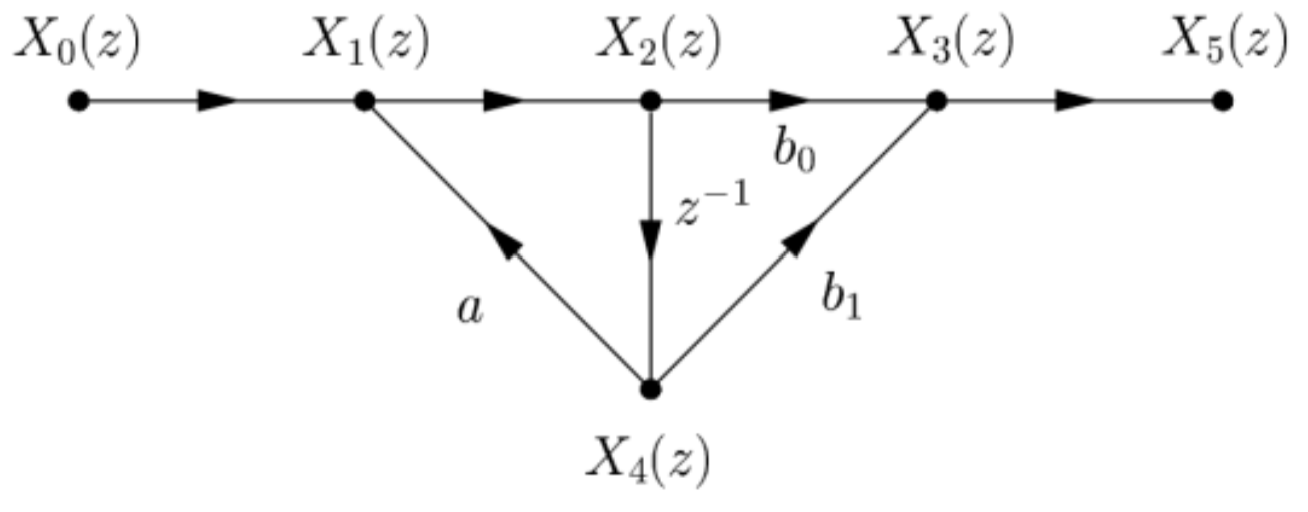
\includegraphics[width=7.5cm]{include/Signalflussdiagramme/SFD_Bsp.png}
    }
\end{tabular}

\subsection{Vereinfachungen}
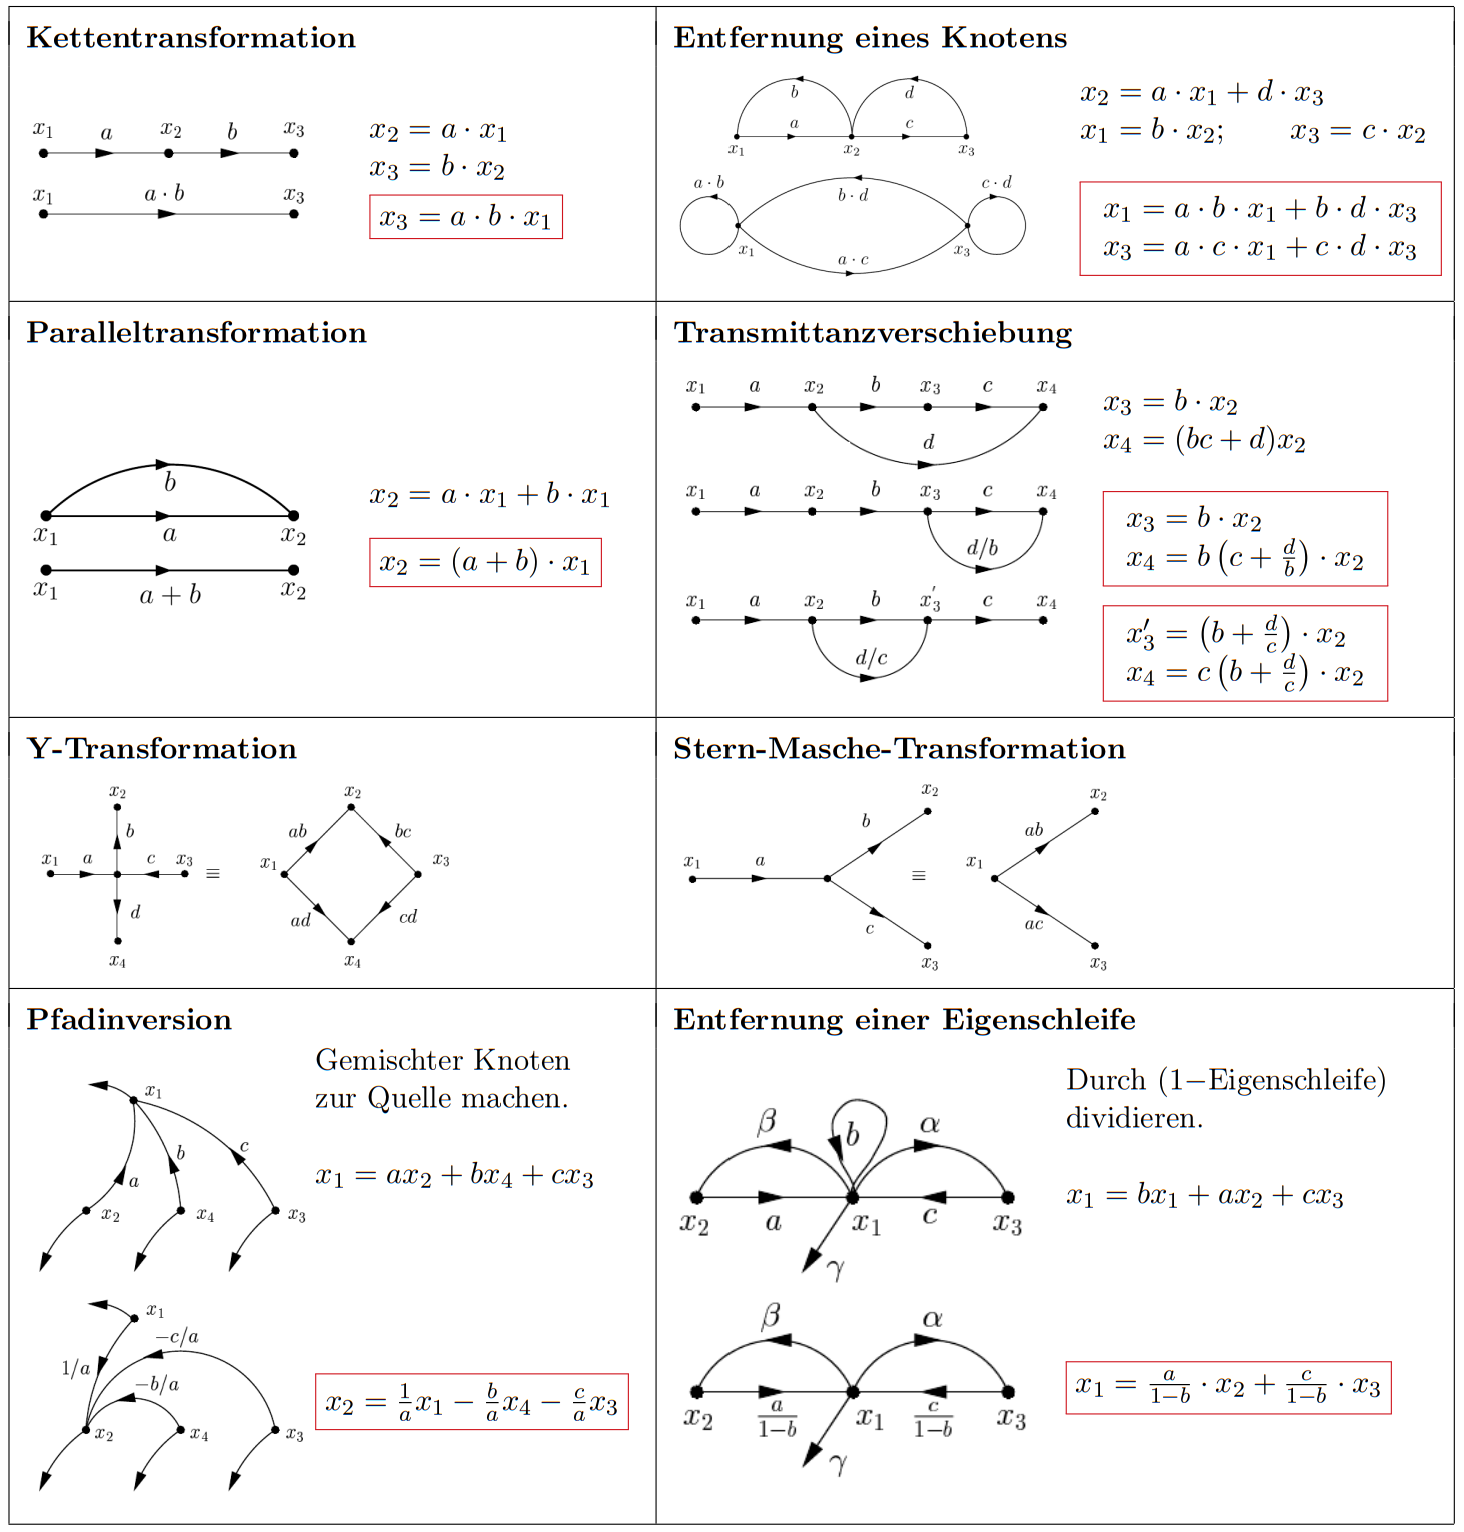
\includegraphics[width = \textwidth]{include/Signalflussdiagramme/SFD_Vereinfachung.png}